\documentclass[review]{elsarticle}

\usepackage{lineno,hyperref}
\usepackage{color}
\modulolinenumbers[5]

\journal{Journal of \LaTeX\ Templates}

%%%%%%%%%%%%%%%%%%%%%%%
%% Elsevier bibliography styles
%%%%%%%%%%%%%%%%%%%%%%%
%% To change the style, put a % in front of the second line of the current style and
%% remove the % from the second line of the style you would like to use.
%%%%%%%%%%%%%%%%%%%%%%%

%% Numbered
%\bibliographystyle{model1-num-names}

%% Numbered without titles
%\bibliographystyle{model1a-num-names}

%% Harvard
%\bibliographystyle{model2-names.bst}\biboptions{authoryear}

%% Vancouver numbered
%\usepackage{numcompress}\bibliographystyle{model3-num-names}

%% Vancouver name/year
%\usepackage{numcompress}\bibliographystyle{model4-names}\biboptions{authoryear}

%% APA style
%\bibliographystyle{model5-names}\biboptions{authoryear}

%% AMA style
\usepackage{numcompress}\bibliographystyle{model6-num-names}

%% `Elsevier LaTeX' style
%\bibliographystyle{elsarticle-num}
%%%%%%%%%%%%%%%%%%%%%%%


\begin{document}

\begin{frontmatter}

\title{Autocategorization}

%% Group authors per affiliation:
\author{Andrew Carnes$^{1}$}
\address{$^1$University of Florida}

\begin{abstract}
In order to maximize the chance of discovering a certain effect, many scientific analyses extract subsets of data from the main data set that are sensitive to the effect. If the effect exists, the data in these sensitive subsets is expected to differ significantly from the null hypothesis. There are many ways to extract subsets, but an optimal method should minimize the global p-value on the null hypothesis given the effect. Call the orthogonal subsets of data categories and the selection of subsets categorization. An optimal categorization enhances the power of the experiment and reduces the data needed for discovery. By specifying a metric corresponding to the expected p-value (given the effect), the optimum categorization may be automated using a decision tree. This paper outlines the widespread uses of categorization in High Energy Physics, describes the autocategorization algorithm, and presents recent uses of the autocategorizer in High Energy Physics. 
\end{abstract}

%\begin{keyword}
%\texttt{elsarticle.cls}\sep \LaTeX\sep Elsevier \sep template
%\MSC[2010] 00-01\sep  99-00
%\end{keyword}

\end{frontmatter}

\linenumbers

\section{Introduction}

Many scientific analyses attempt to rule out a null hypothesis and declare a discovery. In this context, seeing a large enough discrepancy in the data from the null's prediction leads to a low p-value, the rejection of the null, and a discovery. With a model for the null and another for the expected data, the expected p-value can be quantified. An analysis with a lower p-value represents more convincing evidence to rule out the null, and therefore an analysis with a lower expected p-value is considered more sensitive. In addition, a more sensitive analysis requires less data to rule out the null hypothesis. For both of these reasons, optimizing the sensitivity is critical for any scientist.

The expected hypothesis and the null hypothesis determine probability density functions (PDFs) in a many dimensional feature space. However, data sparesly populates high dimensional spaces, and fits in high dimensions are difficult or untrustworthy in practice, so the PDFs are usually compared over a single discriminating feature - sometimes a few - to determine the p-value. Unfortunately, upon reducing to a lower dimensional PDF comparison, the sensitivity of the analysis is often reduced: feature space regions with large discriminating power are combined with those of high probability but low discrimination.

To regain sensitivity, the regions of feature space with large discriminating power need to be extracted. In this way, it makes sense to divide the feature space up into separate regions, called categories, and compare the low dimensional PDFs within the categories to maximize the sensitivity. Typically, the categories are decided using expert knowledge. However, by analytically specifying a metric corresponding to the expected p-value the optimum categorization can be automated. This is separate problem from regression or classification where fit values are applied to different regions of space to minimize some loss function. The goal is simply to divide up feature space to maximize the statistical sensitivity.

Section \ref{chep} presents the ubiquity of human categorization in HEP to motivate the widespread use cases for automated categorization. Next, the autocategorizer algorithm is detailed in section \ref{acat}. Finally, implementations of the autocategorizer in HEP and the resulting improvements are covered in section \ref{app}.

\section{Categorization in HEP}
\label{chep}

%The Large Hadron Collider accelerates protons or heavy ions to nearly the speed of light and steers them to collide in the 
%ALICE, ATLAS, LHCb, and CMS detectors. The different detectors record the collision data, 
%and scientists in the collaborations analyze it to search for new particles 
%and test different theories of physics. 

Many analyses in High Energy Physics (HEP) use categories to improve the statistical power of their investigations. In this section, different scientific analyses from the CMS and ATLAS collaborations of the Large Hadron Collider (LHC) program at CERN are used to illuminate the widespread use of categorization in HEP. Detailed descriptions of the CMS and ATLAS detectors can be found in \cite{cms} and \cite{atlas} respectively. 

The most important contribution of the LHC to date is the discovery of the Higgs boson by the CMS and ATLAS collaborations \cite{atlashiggsdiscovery, cmshiggsdiscovery}. Both of these collaborations made extensive use of categories in the monumental discovery. For example, the Higgs to diphotons analysis of the ATLAS discovery analyzed the diphoton mass in categories based upon the number of converted photons, the number of jets, the pseudorapidity of the photons, and a vector component of the diphoton momentum. In addition, the Higgs to ditaus analysis of the CMS discovery analyzed the ditau mass in categories based upon the number of jets and the transverse momentum of the tau leptons. Other sets of categories are used in these papers for the remaining decay channels. The discovery of the Higgs boson is a significant example of categorization in HEP, but there are many others. 

The 2017 ATLAS search for the Higgs decay to two muons \cite{atlashmumu2017} analyzes the dimuon mass distribution in categories based upon the transverse momentum of the dimuon system, the pseudorapidity of the muons, and a Boosted Decision Tree (BDT) output. The 2017 $t\bar{t}$ dark matter search at CMS \cite{ttdmcms} analyzes the distribution of missing transverse momentum in categories based on the dilepton mass and the number of leptons and jets. The 2017 leptonic supersymmetry search at CMS \cite{susycms} analyzes the missing transverse momentum distribution in categories based upon the number of muons and electrons and their charges. The list goes on. 

The use of categories in HEP is a ubiquitous technique, and wherever this technique is used it could be automated. The autocategorizer algorithm provides an automated method to categorize events that could be used in virtually any HEP analysis. Moreover, the autocategorizer has been used in two CMS analyses to great effect, not only automating the process, but leading to improvements. The implementations and improvements are described in Section $\ref{app}$, but first the algorithm itself is explained.

\section{The Autocategorizer Algorithm}
\label{acat}
This section explains the autocategorization algorithm (autocategorizer) in terms of a binned counting experiment using histograms along a single variable, z. Let $H_o$ be the null hypothesis and $H_1$ be the expected hypothesis -- some trusted theory that probably generates the data. The goal of the autocategorizer is to partition feature space in order to minimize the expected p-value. Minimizing the expected p-value will maximize the chance for discovery if $H_1$ is indeed true.   

Let i label the bin and c label an orthogonal partition of feature space -- a category. Each category has its own histograms. Let $z_{c,i}$ describe the amount in the $i^{th}$ bin of the histogram for category c. Moreover, let $H_o$ predict $z_{c,i} = B_{c,i}$ in each bin for category c and let $H_1$ predict $z_{c,i} = S_{c,i} + B_{c,i}$ in each bin for category c.
\begin{figure}[hbp]
  \centering
  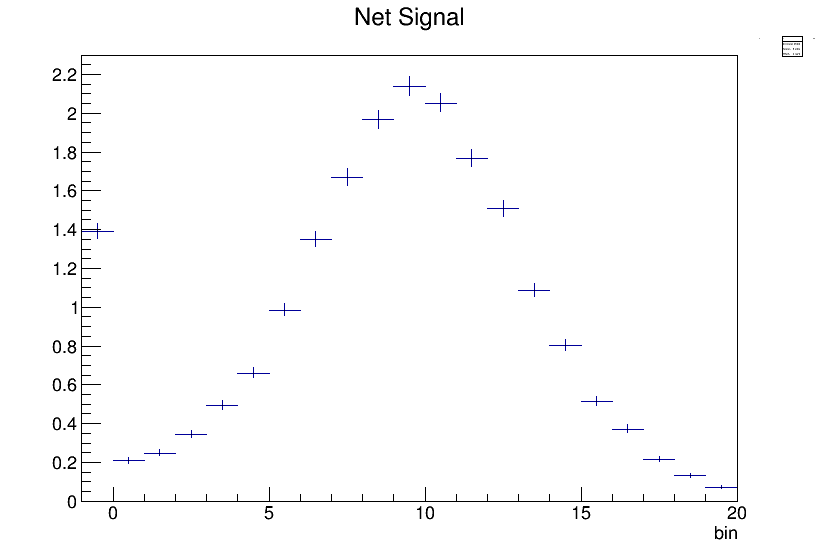
\includegraphics[width=0.49\linewidth]{binning_signal_example.png}
  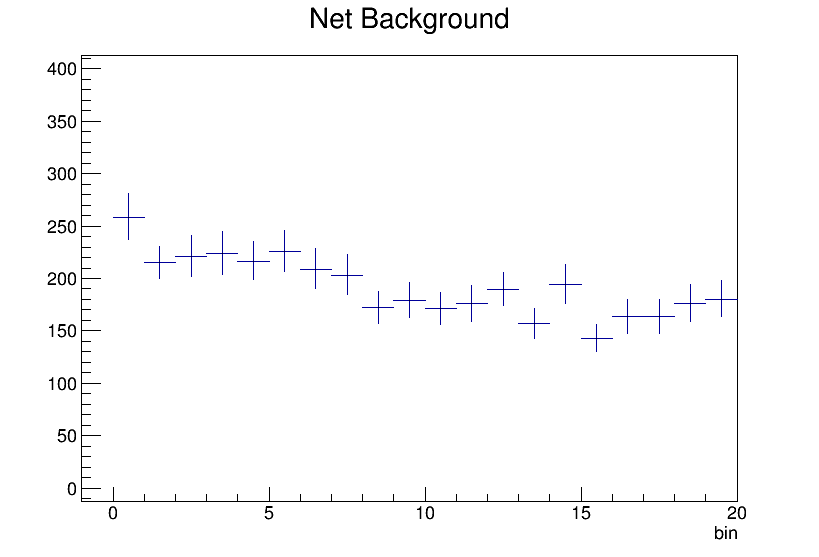
\includegraphics[width=0.49\linewidth]{binning_bg_example.png}
  \caption
  {An example of the S and B histograms in a category. The null hypothesis is given by B, and the expected hypothesis is given by S+B.}
  \label{fig:binning_example}
\end{figure}

The likelihood to observe $S_{c,i} + B_{c,i}$ in each bin when $B_{c,i}$ is expected in each bin provides a statistical measure of the discrepancy between $H_1$ and $H_o$. A low likelihood corresponds to a large discrepancy and a low p-value. Minimizing the likelihood will minimize the expected p-value. Equivalently, maximizing the negative log-likelihood (NLL) minimizes the expected p-value. The NLL for a single category's histogram is given by,  
\begin{equation}
\label{first}
-2log\left( p(z_{c,i}; \lambda_{c,i})/ C_{c,i} \right)  = -2log\left( \prod_{i} Poisson(z_{c,i}; \lambda_{c,i})/C_{c,i} \right),
\end{equation}
where the measured amount in a bin is given by $z_{c,i}$, and the amount expected by the hypothesis is given by $\lambda_{c,i}$. 

The categories are orthgonal, so the likelihoods for each category multiply, and the net NLL is  
\begin{equation}
\label{second}
-2log\left( p(z_i; \lambda_{c,i})/C_{c,i} \right) = -2log \left( \prod_{c,i} Poisson(z_{c,i}; \lambda_{c,i})/C_{c,i} \right) .
\end{equation}
Approximating each Poisson distribution by a Gaussian with $\mu_{c,i}=\lambda_{c,i}$ and $\sigma_{c,i}^2 = \lambda_{c,i}$, leads to a $\chi^2$ variable
\begin{equation}
-2log\left( \prod_{c,i} Poisson(z_{c,i}; \lambda_{c,i})/C_{c,i} \right) = \sum_{c,i}(z_{c,i}-\mu_{c,i})^{2}/\sigma^2_{c,i} 
= \sum_{c,i}(z_{c,i}-\lambda_{c,i})^{2}/\lambda_{c,i}.
\end{equation}
The factor of 2 in front of the log and the $C_{c,i}$ terms standardize the $\chi^2$ variable. To calculate the NLL to observe $H_1$ given $H_o$, $z_{c,i}$ is replaced by $S_{c,i} + B_{c,i}$, and $\lambda_{c,i}$ is replaced by $B_{c,i}$, 
\begin{equation}
{\rm Net~Significance} = \sum_{c,i}(z_{c,i}-\lambda_{c,i})^{2}/\lambda_{c,i} = \sum_{c,i}S_{c,i}^{2}/B_{c,i}.
\end{equation}
Choosing the categories to maximize the net significance will minimize the p-value. 

With the net significance acting as the metric, a decision tree\cite{cart84} can split up the feature space to maximize the metric. The decision tree algorithm greedily builds the optimum categorization by recursively splitting feature space regions into two using hyperplanes. 
\begin{figure}[hbp]
  \centering
  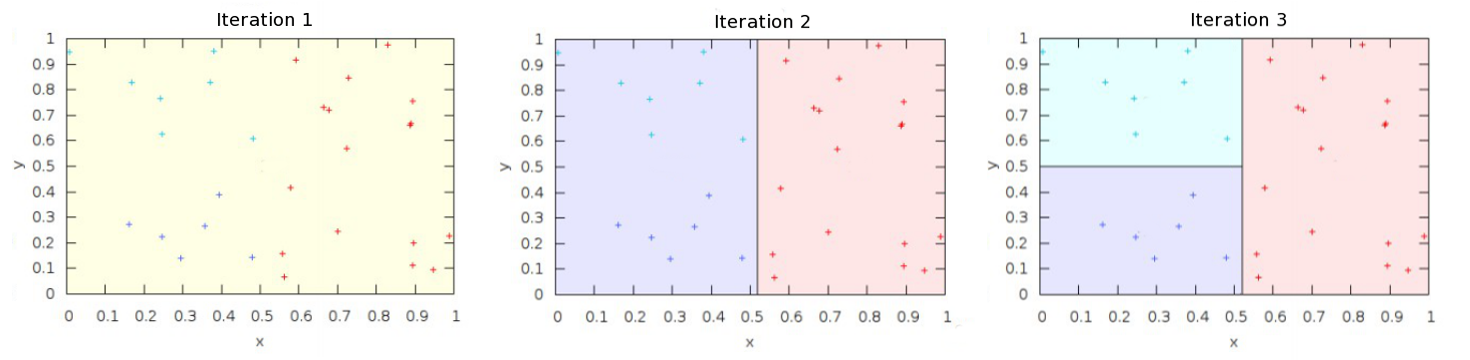
\includegraphics[width=0.98\linewidth]{iter_all.png}
  \caption
  {An example of the autocategorization process for features x,y and three categories. The autocategorizer chooses x=0.52 for the first split and y=0.50 for the second. The colored crosses represent the events that should be grouped together for optimum sensitivity. After three iterations, the categorizer correctly groups those events.}
  \label{fig:iter_example}
\end{figure}
On the first iteration, the autocategorizer calculates the net significance for the inclusive set of all events. The algorithm then searches over the inclusive set, checking all possible split values of the first feature, $x_1$. Events with $x_1$ values less than the split go in one candidate category, and those with $x_1$ values greater than or equal to the split value go into the other candidate category. 

For every split candidate, the algorithm calculates the net significance in the two categories delineated by the split value. The $x_1$ split value that provides the largest gain in significance over the inclusive set is stored along with the value of its gain. The gain is defined in Equation \ref{gain} where c1 and c2 are the prospective categories created from c by splitting on the feature.
\begin{equation}
{\rm Gain} = \sum_{i}S_{c1,i}^{2}/B_{c1,i} + \sum_{i}S_{c2,i}^{2}/B_{c1,i} - \sum_{i}S_{c,i}^{2}/B_{c,i} 
\label{gain}
\end{equation}
The autocategorizer then searches over the second feature, $x_2$, and stores the gain and split value of the best $x_2$ split. The process is repeated for all of the remaining features.

The algorithm chooses to split at the feature value with the largest gain, creating two
categories from the inclusive set of events. At the next iteration, the autocategorizer repeats the procedure for the two new
categories and chooses to split the category that provides the most gain. This process continues, each time greedily choosing to
split the category with the most gain, until the number of categories desired is reached.

The net sensitivity metric used above is just one approximation of the NLL. Other metrics that track the expected NLL/p-value may be used. For instance, adding the Asimov significance \cite{cowan}(Equation 97) of each bin in quadrature is another reasonable approach.

\section{Applications in High Energy Physics}
\label{app}
The standard model of particle physics is an incredibly successful theory, correctly describing all known 
particles and forces -- except for gravity and the neutrino masses. 
The discovery of the Higgs boson (H) \cite{atlashiggsdiscovery,cmshiggsdiscovery,combhiggsdiscovery} 
confirmed that W and Z gauge bosons acquire mass through the Higgs mechanism. 
Soon after, evidence for the Higgs coupling to matter 
was found through the $H\rightarrow\tau\tau$ and $H\rightarrow bb$ decays \cite{cmshiggstau, cmshiggsbb, cmshiggsferm, atlashiggsbb}.
In the standard model (SM), the fermion masses are generated by their coupling to the Higgs field \cite{fromh2muPAS:4-7+quarks}. 
Higgs boson decays to muons and bottom quarks are of particular importance as they extend the study of Higgs couplings to second generation fermions, where deviations from the SM predictions could point to new physics. 

The autocategorizer algorithm has been used at the CMS experiment to set limits on the Higgs boson's rate of decay to two muons \cite{cmshiggsmumu2017} and to two b-quarks \cite{VHbbCitation}. In the $H\rightarrow\mu\mu$ analysis, the autocategorizer improves the expected upper limit on the rate of decay by 13\% compared to human expert categorization. The improvement is equivalent to collecting 27\% more data. 

In the comparison, the human expert categorization of the previous $H\rightarrow\mu\mu$ analysis \cite{cmshiggsmumu2012} is reoptimized for the $\sqrt{s} = 13 TeV$ collisions of run 2, resulting in the expert categorization of Figure \ref{fig:hxcats}. The expert categorization serves as a baseline for comparison. Detailed information on the features can be found in the paper.
\begin{figure}[hbp]
  \centering
  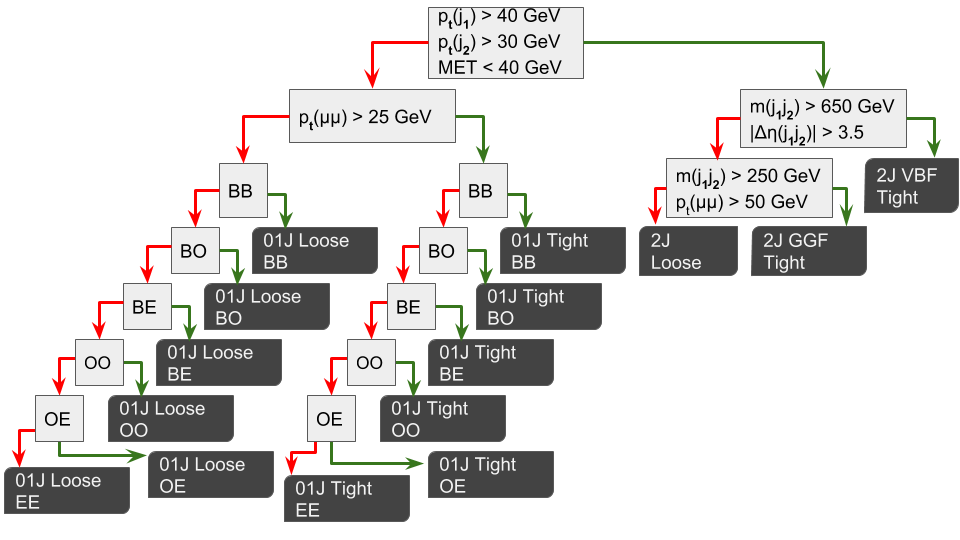
\includegraphics[width=0.98\linewidth]{run1categories.png}
  \caption
  {The human expert categories used as the baseline. B is short for $|\eta(\mu)| < 0.8$. O is short for $0.8 < |\eta(\mu)| < 1.6$ . E is short for $|\eta(\mu)| > 0.8$. These are the barrel, overlap, and endcap regions of the CMS detector. BB requires that both muons are in the barrel, BO requires that one muon is in the barrel and the other is in the overlap, etc.}
  \label{fig:hxcats}
\end{figure}
Running the autocategorizer with the same set of features considered in the 2012 analysis, produces the categories of Figure \ref{fig:autocats}. Histograms of the dimuon mass ($m_{\mu\mu}$) in the different categories are used simultaneously to evaluate the expected upper limit. The SM predictions of $m_{\mu\mu}$ provide the expected hypothesis, while the model for no $H\rightarrow\mu\mu$ decay provides the null.
\begin{figure}[hbp]
  \centering
  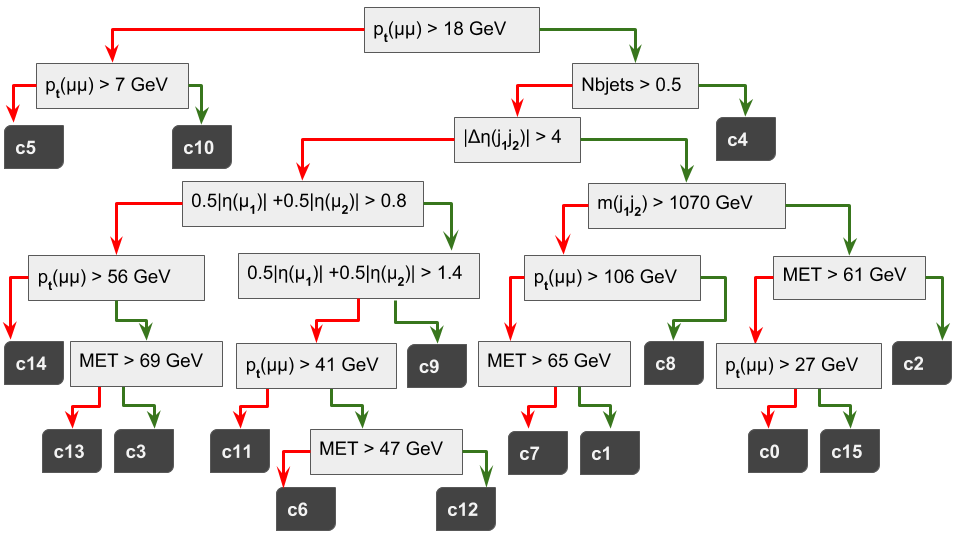
\includegraphics[width=0.98\linewidth]{autocat_categories.png}
  \caption
  {The autocategorizer categories using the same features as the baseline human expert categories. These categories provide a 13\% improvement to the upper limit compared to the baseline.}
  \label{fig:autocats}
\end{figure}

Not only does the autocategorizer improve the upper limit by 13\%, the algorithm also discovers that the previous $H\rightarrow\mu\mu$ analysis overlooked the importance of b-tagging. To quantify the contribution of the b-tagging discovery, the autocategorizer was rerun without b-tagging in the feature set, yielding only 10\% improvement. The test implies that the b-tagging discovery accounts for 23\% of the improvement. 

Categorizing on standard features is only one option. Categorizing on the output score of some machine learning classifier is another. Autocategorizing on the score from a Boosted Decision Tree (BDT) classifier and muon $\eta$ info results in a 23\% improvement in the upper limit and the categories of Figure $\ref{fig:final_categories}$. The improvement is equivalent to 51\% more data. The input features to the BDT can be found in the paper.
\begin{figure}[hbp]
  \centering
  \includegraphics[width=0.98\linewidth]{final_categories_symb-eta.png}
  \caption
  {The autocategorizer categories using the BDT score and the pseudorapidity info of the two muons. Note that $|\eta| = max(|\eta(\mu_1)|,|\eta(\mu_2)|)$. These categories lead to a 23\% improvement to the upper limit compared to the baseline.}
  \label{fig:final_categories}
\end{figure}

The autocategorizer was also used in the $H\rightarrow bb$ CMS analysis to develop a mass analysis. In this case, the autocategorizer was set to maximize the sensitivity metric on $m_{bb}$ by creating categories on the BDT score. Creating categories out of the BDT scoreallows the analysis to use the power of a machine learning classifier while retaining the interpretability of the mass histograms. Moreover, the mass analysis was able to match the expected p-value of the $H\rightarrow bb$ analysis that used the BDT score distributions as the null and expected hypotheses (as opposed to null and expected mass histograms in categories of BDT score). 

%A detailed description of the CMS detector can be found in \cite{cms}. 

%The central feature of the CMS apparatus is a superconducting solenoid of 6 m internal diame-
%ter, providing a magnetic field of 3.8 T. Within the solenoid volume are a silicon pixel and strip
%tracker, a lead tungstate crystal electromagnetic calorimeter, and a brass and scintillator hadron
%calorimeter, each composed of a barrel and two endcap sections. Forward calorimeters extend
%the pseudorapidity ($\eta$) coverage provided by the barrel and endcap detectors. Muons are de-
%tected in gas-ionization detectors embedded in the steel flux-return yoke outside the solenoid.
%A more detailed description of the CMS detector, together with a definition of the coordinate
%system used and the relevant kinematic variables, can be found in \cite{h2mu-paper-22}.

\section{Conclusions}
\label{conc}
%The autocategorizer algorithm automatically maximizes the chance to discover an effect of interest by extracting an optimal ensemble of sensitive regions (called categories) from a multidimensional feature space. 
Categorization is a ubiquitous technique in High Energy Physics (HEP) used to enhance the sensitivity of a statistical analysis. The use of categorization in the discovery of the Higgs Boson as well as other analyses at CMS and ATLAS have been presented. The autocategorizer algorithm presented in this paper automates this categorization process, which has generally relied on human expertise rather than a systematic method. The autocategorizer has been implemented in some recent CMS analyses to great effect. Using the autocategorizer in the search for $H\rightarrow\mu\mu$ improved the sensitivity of the analysis by 13\% alone and by 23\% in conjunction with additional machine learning techniques. These improvements are equivalent to 27\% and 51\% more data respectively. In addition, the recent VH $H\rightarrow bb$ analysis has used the autocategorizer to create an interpretable mass analysis with the power of their BDT score analysis. With the widespread use of categorization in HEP, the autocategorizer algorithm has many opportunities for use in the field. While useful for HEP, the algorithm is a general technique applicable to statistical analyses operating in a many dimensional feature space. 

\section*{References}

\bibliography{mybibfile}

\end{document}
